\chapter{Serverless computing}

\section{Origins}

The growth of cloud computing significantly influenced the way how server management and server application development are perceived. Around fifteen years ago, most of the companies were entirely responsible for managing their software, altogether with the hardware and infrastructure it was running on \cite{RobertsChapin2017}. Around that time, first services capable of outsourcing some part of infrastructure overhead emerged, which started the idea of cloud computing.

Amazon Web Services was one of the first service providers that enabled companies to rent computing capacity by announcing the launch of Elastic Compute Cloud (EC2) in August 2006. It was the first Infrastructure as a Service (IaaS) product on the market that allowed companies to run their server applications on Amazon's machines that are billed per usage time and are available within minutes from requesting new resources.

Leveraging such a service model brings a handful of benefits. It reduces the labour cost by outsourcing hardware management to the provider and infrastructure cost by paying based on actual usage of services. Furthermore, it enables companies to scale the number and type of servers in correlation with the traffic and demand for processing. Finally, it encourages testing new solutions developed by companies by decreasing the lead time, by making the required infrastructure available within minutes instead of months, utilising favourable billing flexibility.

The cost of IaaS solutions is profitable to providers, because of technical improvements done in terms of hardware virtualization and the economy of scale on which they operate. Shortly after other vendors such as Microsoft, Google and DigitalOcean embraced the notion of public cloud by providing services and resources from their own data centers. At the same time, tools like Open Stack enabled companies to use hardware from their own data centers in the same way, forming the idea of private cloud.

The next step in the cloud evolution is Platform as a Service (PaaS). As a layer on top of IaaS, it adds operating system to the outsourced infrastructure stack enabling to deploy the application code directly. In that model, the platform takes responsibility for managing the operating system as well as monitoring and running the application. Google App Engine, AWS Elastic Beanstalk and Heroku platform can be distinguished as most popular PaaS solutions, while one of the most frequently mentioned self-hosted variant is Cloud Foundry.

The growth of containerisation technologies introduced another type of service called Container as a Service. Technologies like Docker allowed developers and system administrators to deliberate more clearly on the application requirements and separate it from the operating system. Solutions such as Marathon running on top of Mesos and Kubernetes introduced a possibility to manage and orchestrate containers on self-hosted machines. The services provided by cloud vendors include for example Google's Compute Engine or Amazon's Elastic Container Service (ECS) or AWS Fargate. With the growing popularity of Kubernetes, dedicated services leveraging that platform such as Amazon Elastic Kubernetes Service (EKS) and Google Kubernetes Engine (GKE) emerged.

Each of the described services are next generations of infrastructure outsourcing, which raise the level of abstraction from the development perspective and hand off more and more responsibility related to infrastructure management to the cloud vendor. Despite the fact, for each of the mentioned services the smallest unit of processing is some sort of server application or running application process in the virtual machine or within the container.

Serverless is considered as a next step in the cloud computing progression. The term serverless was one of the first used by Ken Fromm in his paper \cite{KenFromm}. It describes the notion of architecture migration from monolithic applications running on servers into distributed systems that consist of multiple components, processes and data stores with the goal to perform various tasks and process numerous flows. The serverless architecture enables developers to make a mindshift accordingly. Computing resources can be used as services, which makes it possible to shift thinking from the servers level to the tasks level, taking away the complexity of infrastructure management. The servers are still used underneath, but developers don't need to worry about managing them any longer.

Such an architecture model was leveraged firstly by mobile applications built on top of hosted database solutions such as Parse (later acquired by Facebook) and Firebase around 2012 (obtained by Google). Nonetheless, the most significant event shaping the serverless architecture was the announcement of AWS Lambda in 2014, altogether with the introduction of API Gateway in 2015. By the middle of 2016, major cloud vendors such as Microsoft and Google embraced the serverless architecture approach and started offering their services for developing serverless applications.

\section{Defining serverless}

Despite the fact that the idea of serverless computing emerged about a decade ago, it has been already widely adopted by leading cloud providers. Currently it covers a range of technologies, components and cloud services. Nevertheless, there is no clear and concise view on what ''serverless'' is. Various vendors, organisations and research groups tried to define what the serverless term means for them.

Cloud Native Computing Foundation of the organization working towards standardisation of numerous cloud-related technologies and components. It maintains a sustainable ecosystem for cloud native software by bringing together and collaborating with various members of the cloud community. According to ''CNCF Serverless Whitepaper'' \cite{CNCFServerless}.

\begin{quotation}
Serverless computing refers to the concept of building and running applications that do not require server management. It describes a finer-grained deployment model where applications, bundled as one or more functions, are uploaded to a platform and then executed, scaled, and billed in response to the exact demand needed at the moment.
\end{quotation}

Another definition considering the serverless service capabilities can be found in a booklet made by Mike Roberts and John Chapin titled ''What is Serverless?'' \cite{RobertsChapin2017}.

\begin{quotation}
\noindent A Serverless service:
\begin{itemize}
    \item Does not require managing a long-lived host or application instance
    \item Self auto-scales and auto-provisions, dependent on load
    \item Has costs that are based on precise usage, up from and down to zero usage
    \item Has performance capabilities defined in terms other than host size/count
    \item Has implicit high availability
\end{itemize}
\end{quotation}

The cited definitions contain insightful information about features of serverless architecture and capabilities of its components. These can be summarized as follows:

\begin{itemize}
    \item Serverless architecture defines the new model of developing and executing workloads. The application consists of multiple serverless components configured together to run the business logic within the application code, designed to be executed in a serverless environment.
    \item It does not require to maintain, provision and monitor servers and applications. Serverless does not mean that there are no servers - the overhead of managing them is handed off to the cloud provider.
    \item Deployment model is more granular. Having the application built from multiple components configured to work together, the deployment can update only selected ones.
    \item Platform is responsible for provisioning and executing the applications. With a large resource pool maintained by cloud provider and the possibility to quickly allocate it, the solution can be scaled automatically to the current load requirement almost instantly.
    \item The cost is proportional to the resource usage. Each of the components involved in performing the computation is billed granularly, with an accuracy to hundreds of milliseconds or number of executed operations, with no cost when being idle. Executing hundred operations in parallel will cost the same amount of money as running that workload sequentially.
    \item The performance is not related to the host size. Some of the cloud providers enable customers to choose how much memory and CPU can be allocated for the environment. Nevertheless, the configuration is abstracted from the capabilities of the underlying machine that is used as an application execution environment.
    \item The serverless components are built with high-availability and fault-tolerance in mind. Despite the fact that developers are no longer concerned with servers, the underlying vendor's machines can still fail. When using serverless services we expect that cloud vendors will provide transparent high availability for its services. Although, as developers it may be necessary to handle some errors and failure occurrences properly.
\end{itemize}

\section{Serverless components}

When considering the serverless architecture we refer to a range of technologies provided by cloud platforms. Two different areas can be distinguished, defining two distinctive components:

\begin{itemize}
    \item \textbf{Backend as a Service} refers to third-party services or generic components capable of replacing some part of a server side application, that has been previously developed internally or self-provisioned. It exposes an API which allows for integrating the component with the rest of the application.
    \item \textbf{Function as a Service} is an event-driven execution environment for running application code within stateless and ephemeral containers with strictly limited execution time.
\end{itemize}

Aforementioned components used simultaneously enable developers to build fully-fledged solutions utilising serverless architecture and are offered together within a single cloud platform.

Even though presented areas serve different roles, they share common features and capabilities. These could be listed as follows:

\begin{itemize}
    \item Require no resource management and are entirely provisioned by cloud provider
    \item Billing is proportional to actual usage
    \item Utilise the event-driven model for processing
    \item Underlying platform ensures automatic horizontal scaling, high availability and fault tolerance
\end{itemize}

\subsection{Backend as a Service}

The concept of Backend as a Service (BaaS) gathers various domain-generic, repeatable application components capable of replacing some part of application logic or providing some functionality. They can be accessed and integrated into developed applications through API defined by its provider.

Taking into consideration most popular requirements of various applications, the majority of them need to store and manage the data. Depending on the requirements the information should be stored in a structural way in databases or can be stored regardless of their shape in file storage service. For teams developing mobile or web applications it is convenient to rely on some third-party service to store and access the data directly from the application. Services like Google's Firebase meet such requirements and give access to the database entirely managed by a cloud vendor. Depending on the complexity of developed product it may be required to incorporate some more advanced components to process required tasks or flows reflecting the business logic of application. Mechanism serving as notification services, exposing some publish-subscribe capabilities for defined events could be applicable in that case. It is essential to notice that such components are replacing previously self-hosted components such as databases or other data stores, message-brokers or other services responsible for processing data streams incoming from various sources.

Looking closer from the application logic point of view, there are also repeatable functionalities implementations that can be extracted and reused across multiple developed applications. Most of the products will require some features enabling users to manage their identity and associated permissions. Most of the time, the capabilities will be not only limited to registering and logging users, but it will also include integrations with other services as identity providers. Managing and sending emails can be considered as another functionality that can be extracted into separate component from the code perspective and reused in other applications. Products such as Auth0 (serving as fully featured authorization and user management service) or Mailgun (capable of managing and processing emails) makes it possible to replace entirely the repeatable part of business logic.

% TODO:rb update chapter reference
Specific components and services that can be classified as Backend as a Services will be covered in more details in chapter ... when analysing services provided by leading cloud vendors. All of the mentioned components enable developers to create fully fledged applications and services similar to the solutions built using self-hosted component equivalents. The difference is that mentioned components are characterized by capabilities of the serverless architecture. They are provided by cloud vendors, who take responsibility for managing, provisioning and scaling them depending on the demand. Moreover, the possibility to replace the repeatable application features by utilising third-party services enables developers to iterate faster and shorten the lead time.

\subsection{Function as a Service}

The second area refers to Function as a Service (FaaS) that serves as an environment for executing application code. It introduces a new architectural approach in terms of developing, structuring and deploying the application logic, which is oriented towards individual tasks and operations.

Mike Roberts briefly described the idea of FaaS \cite{MartinFowlerServerless} based on the definition of AWS Lambda \cite{AWSLambda}, which is currently one of the most commonly used implementation of a Function as a Service platform. Based on his summary several main features of FaaS can be highlighted:

\begin{itemize}
    \item The main idea of FaaS is to run application code without managing servers and application processes. It is a common feature with other approaches like CaaS or PaaS, where the responsibility for managing applications is placed on the cloud vendor. However, the key difference with FaaS is the fact that the function execution time is strictly limited in contrast to long-lived processes existing in aforementioned services.
    \item The functions are invoked and executed on the underlying platform in response to specific events occurring or incoming into the system. Based on that cloud provider handles resource allocation and runs the function code in an ephemeral container, created based on runtime needs. These are destroyed shortly after the event is processed by the application logic in the function. Together with limited execution time it is a significant architectural restriction for the FaaS model.
    \item Given the fine-grained execution model, horizontal scaling can be easily and automatically handled by the cloud provider. When there is an increased traffic in the system, the platform responsible for executing functions allocates resources to create and run more functions, which will be capable of processing the increased traffic. An analogous situation takes place when there is no traffic, therefore there is no need to allocate resources for running functions code.
    \item As a consequence of greater granularity of application code and managing the function execution by cloud provider, the deployment process differs from the traditional system. Each function can be independently packed and uploaded to the FaaS platform, which takes responsibility for executing it.
    \item Most of the cloud platforms do not require to use neither predefined framework nor programming languages. Although cloud providers define the list of environments and languages that are supported by the platform, any process that is bundled into the artifact and can be executed from it is capable of processing the incoming event.
\end{itemize}

Selected aspects of Function as a Service architecture are covered in more details based on ''CNCF Serverless'' whitepaper \cite{CNCFServerless} in the following sections.

\subsubsection*{Function lifecycle}

Before analyzing the execution model in more details, it is important to examine the deployment process accompanying the development of a function. Alongside with providing the function code, the developer is responsible for specifying one or more events upon which function will be triggered. Additionally, metadata defining for example the function version, environmental variables, execution role and other configuration parameters can be defined. The function and specification prepared in that way is uploaded to the cloud provider and processed by a dedicated builder entity, resulting with a function artifact (depending on the cloud platform and selected runtime it can be a binary file, container image or a package). Next, it is deployed on a cluster managed by a FaaS controller responsible for provisioning, controlling and monitoring function instances based on incoming events.

\begin{figure}[h]
    \centering
    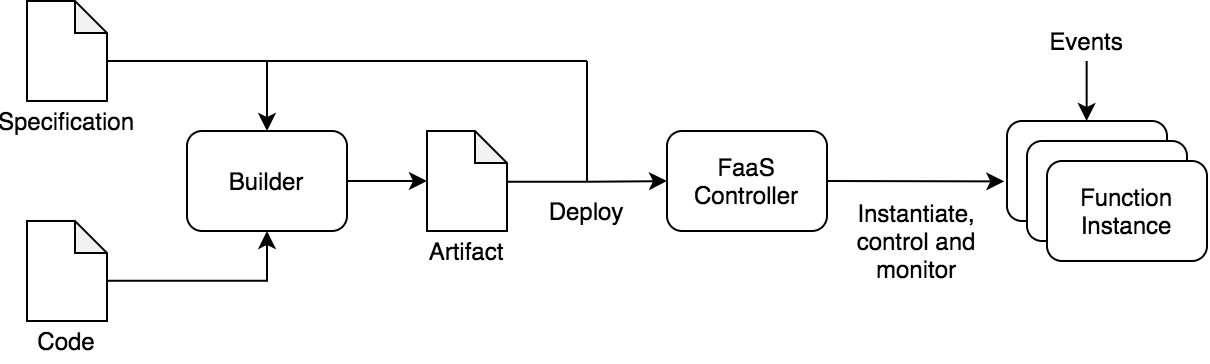
\includegraphics[width=0.8\textwidth]{assets/02-serverless/ServerlessDeployment.png}
    \caption{Function deployment and invocation process}
    \label{fig:function-deployment-and-invocation-process}
\end{figure}

Furthermore, the serverless platform may provide additional actions related to function management such as executing, publishing, updating and deleting the function or its metadata. Also, a particular version of the function can be labeled or aliased, which can come in handy when operating the serverless system on a larger scale. Logs and statistics are gathered alongside function execution.

The function is executed in an event-driven model and within strictly limited duration. The whole process begins when an event triggering a particular function is dispatched. It is detected and registered by an underlying serverless platform. The controller responsible for managing function execution looks for functions associated with incoming events, gets its code and configuration and allocates an adequate amount of resources from the managed resource pool. The new execution environment is created inside a lightweight, ephemeral container and language runtime for the function is bootstrapped. When it's ready, the triggering event is redirected and processed by the application logic contained in the function code.

The results of computing are sent back to the event dispatcher. Other, newly created events can be dispatched during function execution. The computing duration is limited by the majority of service providers up to a few minutes, after that the computation is completed with timeout. At the end the lightweight container containing the execution environment is destroyed.

Most of the providers delay the container deletion for longer than a couple of minutes due to optimisation related with reusing the same container instance when the next event occurs in the system. Reusing an already initialised execution environment is called a ''warm start'' and allows to reduce the startup latency related to resource allocation and runtime preparation. The opposite situation takes place when the new container instance needs to be initialised and the host process needs to be created. Most of the time it requires additional time impacting the request processing duration - it is called ''cold start''.

\begin{figure}[h]
    \centering
    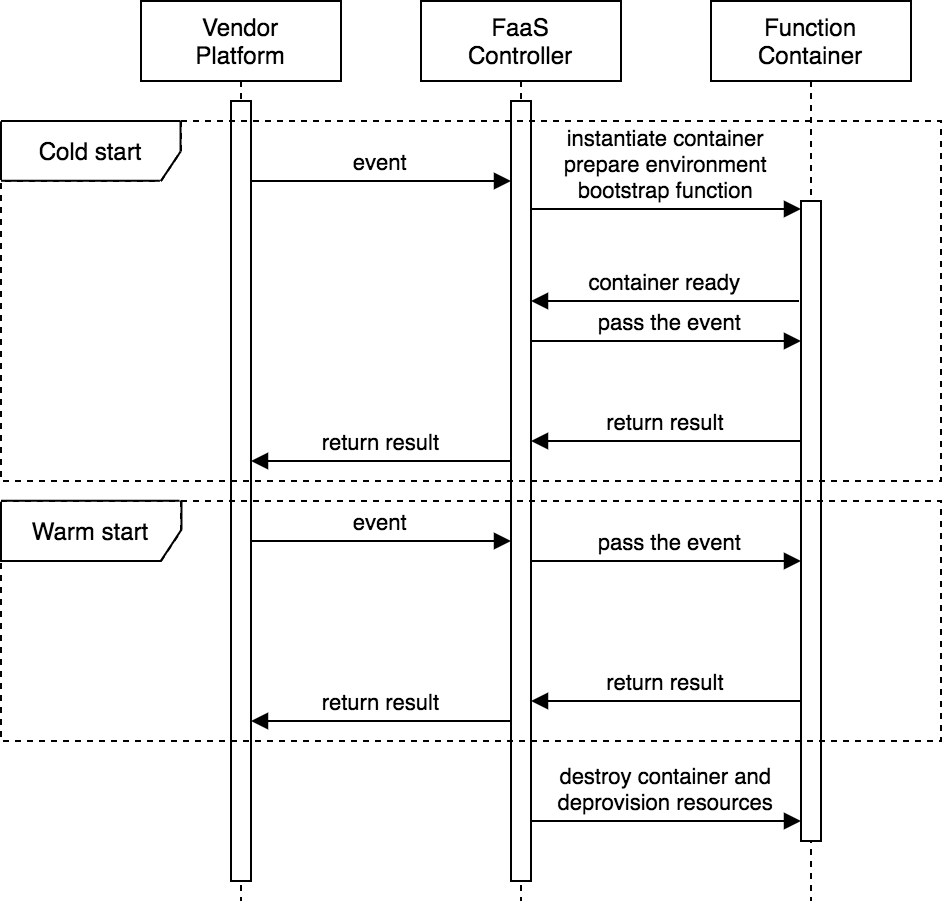
\includegraphics[width=0.7\textwidth]{assets/02-serverless/ServerlessExecution.png}
    \caption{Function execution process considering ''cold start'' and ''warm start''}
    \label{fig:function-execution-process}
\end{figure}


\subsubsection*{Function environment}

The characteristic of the function environment has been already drafted during description of the function lifecycle. Due to improvements in the software virtualisation area, cloud vendors can benefit from efficient and elastic management of large resource pools. It enables vendors to allocate efficiently lightweight and ephemeral containers, serving as an execution environment. Each of them is initialised to execute code of one of the functions at a time and it is destroyed shortly after, releasing the resources to the common pool. Even though containers can be reused for the optimisation purposes when handling subsequent events occuring in the system, it is not guaranteed by the serverless platform and should not be taken for granted by developers, that some data could be preserved for subsequent invocation.

Such an architecture leveraging stateless containers allows for automatic horizontal scaling. When multiple concurrent events occur within the system, the platform is capable of creating a separate container to process each of them independently. In order to handle spikes of traffic effectively, quick provisioning of the containers and reducing their startup latency is required and it is a purpose many research works and improvements made by both researchers and cloud vendors

As mentioned before, ephemeral containers are dismissed shortly after the execution alongside with their internal state. For some types of computing it would be desirable to preserve that state. To address that issue, external components need to be introduced to persist the data. Nevertheless, it introduces the need to communicate with some external service and it is often associated with additional delays resulting from the communication overhead.

\subsubsection*{Function invocation}

The serverless architecture utilises an event-driven processing model. The developer's task is to define configuration that maps events coming to the system with appropriate functions. Each of dispatched events can trigger one or more functions as well as each function can be invoked by one or more predefined events - there is a many-to-many association between function and event sources. The mapping can also refer to a particular version of the function or alias, which can greatly simplify the deployment process by replacing the function code for a given alias without modifying the configuration.

Various data sources can be divided into several categories among which we can distinguish:

\begin{itemize}
    \item Endpoint Services - Most of the time associated with API Gateway components, which introduces mapping between request coming from APIs, such as REST or Websocket and associate them with corresponding functions
    \item Storage Services - Category includes numerous BaaS components provided by a cloud vendor like databases, file storage or cache services. Events can be emitted based on operations performed on the data such as creation, deletion or modification of it.
    \item Messaging Services - Services providing mechanisms for data streaming, message brokers or various services sending notifications.
    \item Scheduled events - That category include services capable of emitting events periodically at a given time or at a selected interval
\end{itemize}

Based on the use case, several invocation types can be differentiated:

\begin{itemize}
    \item Synchronous Request - Includes cases when the client sends a request and waits for the response. It is used most frequently for HTTP requests.
    \item Asynchronous Message Queue Requests - Refers to events emitted from various data sources when messages are published to some exchange that later distributes it to other subscribers. Messages are delivered exactly once without strict ordering.
    \item Event Streams - Are based on streams of messages, logs or files. Sequence of record is most of the time partitioned into several shards.
    \item Batch Jobs - Refers to jobs that can be splitted into smaller tasks and processed in parallel by multiple functions. The entire process is completed when all subsequent tasks are finished.
\end{itemize}

\section{Benefits and challenges}

The emergence of serverless architecture has met with great interest from various software architects, developers and companies that noticed numerous advantages of this approach. In addition to the promise of significant cost reduction, the development and operational opportunities and reducing time to market are just a few of the benefits that serverless introduces.

Nevertheless, the serverless architecture also has many disadvantages, inherently connected with its nature. Some of them have been addressed by various cloud vendors working towards improving their services and mitigating the problems. Despite the fact that many companies already adapted it, the technology is still not fully mature. There is much research ongoing in the various areas conducted by both researchers and cloud providers.

Based on the reports and articles discussing the advantages and drawbacks connected with the serverless architecture \cite{MartinFowlerServerless} \cite{BerkeleyServerless} \cite{ServerlessComputingSurveyOfOpportunitiesChallengesApplications} \cite{LeveragingServerlessCloudComputingArchitectures}, the benefits and challenges of the serverless architecture have been presented. The challenges have been divided into three distinctive categories.

\subsection{Benefits}

\subsubsection*{Reduced development and operational cost}

Serverless is essentially another step in the process of infrastructure management outsourcing, similar to IaaS and PaaS. Instead of requesting resources, developers can provide an artifact including code to be executed and the cloud platform is responsible for provisioning the resources and executing the code, based on defined triggers' configuration. The responsibility of managing the servers, databases and application execution is transferred to the cloud provider \cite{BerkeleyServerless}. The favourable and competitive prices are available due to economy of scale, in which one vendor is running thousands of predefined services, effectively sharing the infrastructure among the customers.

The labour cost connected with the serverless architecture is also reduced, because there is less work related to managing the serverless solution, compared to the self-hosted alternative. There is no need to setup, maintain hardware and restore it to proper condition in case of failures - new resources can be allocated and be ready to work with, within a moment from requesting it. The development cost is also reduced due to the frequent usage of BaaS components, replacing the application elements that were previously developed in-house, now can be incorporated with the application logic. An example of such approach is aforementioned Auth0 providing the authentication capabilities or Firebase, enabling client applications to directly communicate with server-side databases, accordingly providing proven authentication mechanisms for different types of users and removing much of the database administration overhead \cite{MartinFowlerServerless}.

\subsubsection*{Autoscaling with proportional cost}

The serverless billing model refers to paying proportionally to the time resources are used, instead of calculating the cost based on the size of cloud resources as in IaaS or PaaS offerings. By tracking the load with a greater fidelity, scaling up quickly in case of increased demand and scaling down in the absence of it, customers are actually charged for the time the code was executed rather than the resources used to execute their software \cite{BerkeleyServerless}.

Additionally with the greater granularity, only the components affected by increased demand can be scaled accordingly compared to the conventional serverful computing. The serverless processing is characterized by the instant horizontal scaling, which is an ability to parallelize heavy workloads almost instantly on demand and deprovisioning resources shortly after, that is an automatic process handled entirely by the cloud provider. It enables companies to shift from the capital expense to the operational expenses when running their software, which removes the need to invest beforehand in costly hardware before the application or service is created and deployed \cite{LeveragingServerlessCloudComputingArchitectures}.

The cost reduction is most visible when the service has to process the occasional or inconsistent traffic. In the first case the processing will be executed based on the event, billed accordingly to execution time and not paying for idle, which is significantly more efficient compared to the self-hosted solution in which some server is running the application all the time. When running the application in the second case, it may be necessary to have enough hardware to handle the highest demand to ensure the running service is capable of handling all the requests. With the serverless solution the cloud provider is responsible for scaling to handle the demand. The customers pay only for the additional time hardware was computing to satisfy the higher traffic. Comparing to provisioning virtual machines there is no risk of overprovisioning (when demand is handled on time, but the resources are not fully utilised) or underprovisioning (when the average processing capacity is optimised, but the highest traffic may not be handled on time or even not at all). These examples are deliberately picked to showcase the significant cost savings of serverless, but on the other hand when the traffic shape is making a good utilisation of running servers, the cost of using serverless technologies can be higher. Lastly considering the serverless model, any performance optimisations making the function execution shorter or reducing the number of requests to some other BaaS component can accordingly reduce the cost \cite{MartinFowlerServerless}.

\subsubsection*{Easier operational management}

Considering the scaling is automatically handled by the cloud vendor, there is no need to hire qualified administrators to manage and scale the application and make sure that the service is running properly, which leads to further cost reduction. The packing and deployment process for serverless solutions is also simplified compared to deployment of new versions of software to the servers. There is no need to manage some scripts or specified software responsible for managing the deployment, the serverless solution can be packed, zipped with appropriate configuration and deployed to the cloud, where the cloud vendor handles the rest of the process. In the fully serverless solutions the system administration role can be effectively minimised by the serverless platform when embracing the proper process automation \cite{MartinFowlerServerless}.

\subsubsection*{Development opportunities}

Serverless solution is appealing, because of the possibility to reduce the cycle time. The focus of development can be put on the business logic and developing the product instead of managing the infrastructure.

The serverless architecture brings new architectural opportunities and provides some interesting architectural properties. For example the automatic horizontal scaling brings yet another benefit - the software architects and developers no longer need to think about designing the solution to ensure the scalability, cause it is provided out of the box by the cloud platform. Similar situation can be noticed for the implicit failover. There is no need to run another instance to pick up the computation once the first one fails. FaaS handles implicit failover by retrying the execution on newly provisioned functions once the initial on crash \cite{LeveragingServerlessCloudComputingArchitectures}.

The cloud platform provides various BaaS components, giving a possibility to incorporate and integrate them with the developed solution. They are giving various capabilities not only related with authentication, storing data or exchanging messages in a publish-subscribe manner, but also give some more sophisticated services including documents and image processing, generating transcriptions or incorporating machine learning for advanced prediction. It gives the opportunities for developers to look at a vast area of new possibilities with a matter of integration and configuration of some of the services.

It is especially beneficial for agile teams gearing towards lean and agile processes, by reducing time to market, which is understood as the time from an idea until the product is available for the customers. Having the better granularity of code and without the need to manage the infrastructure, the new version of a service can be released more frequently, moving towards the idea of continuous deployment. Along with the granular billing model the companies can try out new solutions with minimal cost and friction. The new experiments can be deployed within a moment since the development is completed, enabling the product owners to set the mindset of continuous experimentation. The proof of concept feature with the limited traffic will cost proportionally low or could be even free if the resource utilisation fit into the free tier provided by some of the cloud providers \cite{MartinFowlerServerless}.

\subsubsection*{Greener computing}

The growth of awareness about environmental problems has influenced the way the data centers are built. To fulfill their energy requirements cloud providers host their data centers near the renewable energy sources to reduce the fossil-fuel emission. Contrary to the typical data centers, which are delivering only some percent of their real computing output, while some of the servers can be running idle inefficiently consuming the energy.

Cloud infrastructure partially mitigates that problem, because the companies are renting the computing resources based on the demand, rather than provisioning the servers on their own, especially when these are run without adequate awareness about the capacity management. When using IaaS, PaaS or self-hosted solutions most frequently the users are responsible for scaling the services, preferably overprovisioning the resources which leads  to inefficient energy utilisation. The cloud provider takes the responsibility for the serverless solutions by provisioning the compute resources and handling the capacity decisions to fulfill the needs, leading to far more efficient resource and energy utilisation across data centers and reducing the environmental impact \cite{MartinFowlerServerless}.

\subsection{Challenges related to the nature of serverless architecture}

\subsubsection*{Function state management}

As mentioned before the FaaS are effectively stateless and due to that have a significant limitation when it comes to the local state. It should be assumed that the state from one invocation will not be available in another invocation of the same function, which is connected with the lack of control over the ephemeral container function is running in. To share state between subsequent function execution it should be preserved in some external component like database, cache or external object storage, which introduces significant communication overhead leading to latency increase \cite{MartinFowlerServerless}.

It highlights that some types of computation relying heavily on fine-grained state sharing may not be suitable for the serverless model. Two distinctive types of storage needs to be addressed. First of them is a low-latency ephemeral storage enabling to transfer data between functions and maintain the application state during application lifetime. Once processing is finished, the state can be discarded. To achieve that some in-memory cache with optimised network and low latency operations can be considered. Nevertheless, the main challenge there is to provide automatic scaling, allocating and freeing resources and ensure access protection together with performance isolation. The second type refers to durable storage, as a long-term data storage with mutable semantics of a file system. It should also be transparently provisioned, ensure proper level of isolation, security and performance predictability, but contrary to ephemeral storage the data should be durable and the removal should be explicit along with maintaining low cost \cite{BerkeleyServerless}.

\subsubsection*{Function communication and data transfer}

The service built using the serverless architecture is essentially a composition of many functions and BaaS components working together to provide the desired functionality. To achieve that, functions need to communicate somehow  and exchange the data. In other cloud services communication can be attained through network addressing, but in serverless architecture functions are ephemeral and anonymous. The function-level addressing is not available and they need to communicate through intermediate storage or messaging service introducing additional latency and which can be pretty expensive with finer-grained communication patterns. Additionally, the fact that functions can be allocated and load balanced according to the current utilisation of resources in the data center impacts the performance when the data needs to be transferred to the function. Due to that the data caching in a serverless environment can be more difficult to be implemented in an effective way since the functions are placed and executed independently \cite{ServerlessComputingSurveyOfOpportunitiesChallengesApplications}.

Some of the communication patterns known from machine learning or big-data analysis software like broadcast or aggregation require sending more messages and can be less performant when implemented in a serverless architecture. Compared to the software running on virtual machines the tasks can share a copy of the received data and perform local aggregation to limit the message overhead and amount of data being sent. Moreover, the serverless component utilises most frequently some intermediate component working in a producer-consumer pattern to send the data, which introduces additional communication delay. Due to lack of addressability the functions are unable to communicate directly, for example calling one another when the data is present or coordinate some distributed operation \cite{BerkeleyServerless}.

To address that problem cloud providers could enable developers to assign the group of functions to the same machine instance, reducing the data exchange overhead or compute the communication graph to place functions efficiently, but it would reduce the flexibility of cloud providers and data centers utilisation. Some of the offerings such as AWS Step Function or Azure Durable Functions try to address the function orchestration problem, by running a sequence of lambda functions as event-driven workflow and efficiently maintain the application state between the subsequent invocations.

Some of the approaches of various practitioners consider some sort of hybrid solution to address the problem of externalized state constraint and lack of function addressability. The low-latency application can be run as regular, long-running servers handling the requests and keeping the context in local memory, handing off the fully contextualized requests to FaaS executed concurrently to process some computation without need to lookup for external data.

\subsection{Cloud platform and vendors challenges}

\subsubsection*{Vendor dependency}

As with any outsourcing technology some control of the system is given up to the service provider and it is no difference with the serverless. The cloud vendor can put some constraints on how the clients use their services in form of unexpected limits or API changes to be more likely to deliver the reliability on its side. Similarly when using BaaS components, developers no longer need to implement and maintain them, but it is not guaranteed that the external services will be running without some issues or unexpected failures. If the cloud platform would satisfy the needs of hundreds of customers or the smaller group, it will most probably choose the majority to ensure accountability of services \cite{MartinFowlerServerless}.

\subsubsection*{Vendor lock-in}

The cloud provider selection is a significant decision when building some service using the serverless architecture not only due to their offerings, but also due to differences in their services implementation that makes the further shift harder or even almost impossible without major changes. When taking a closer look at the function invocation semantics, each of them depicts the different interface and events triggering it. The divergence also occurs on the level of BaaS components which expose various behaviours and API which may even require to change the architecture solution in some cases. Moreover, operational tools related with deployment, logging, monitoring and configuration management will most probably differ and require migration.

When migrating the serverless solution from one of the cloud providers to another one, some parts of the system can be translated more easily, but others can have a significant impact on the whole architecture of the developed solution. For example porting of some function code between cloud platforms won't be possible without migrating other chunks of the architecture. Some companies adopt multi-cloud approaches leading to developing and operating the application in a way that is agnostic to the cloud vendor. Most frequently it is a more costly solution, which makes it impossible to apply benefits, optimisations and more specialised components provided by the cloud vendor \cite{MartinFowlerServerless}.

\subsubsection*{Startup latency and platform improvements}

Serverless functions have much lower startup latency than the application executed on the virtual machines, but because of the frequency of using new function instances the low startup time is crucial to provide efficient processing. The function startup time consists of scheduling and allocating the resources to run the function, establishing the environment for code execution and initialising the libraries and data structure to run the function code.

When the function is executed for the first time after a longer period of inactivity or when a new version is deployed, the function bootstrapping process will consist of all of the steps forming aforementioned "cold start". Providers already noticed that resources and environment of the function containers can be reused to save some of the bootstrap time. Nevertheless, the most noticeable latency related to the full function setup has a significant impact on the service performance from the user point of view \cite{BerkeleyServerless}.

Different approaches are currently available to mitigate that problem, but they are coming with an additional cost. The serverful instances can handle low-latency applications well, because they are always running and ready to serve the traffic. Similarly, function can be pre-warmed regularly to ensure the resources and environment is ready to satisfy the incoming request. AWS Provisioned Concurrency is one of the dedicated extensions to the AWS Lambda service, while Serverless Framework includes some plugin enabling that by registering scheduled events that keep functions warm.

Another factor limiting the serverless function execution is constrained execution duration. Various FaaS offerings from the biggest cloud providers limit the execution time to elastically manage their resource pool. Beyond that cloud vendors could increase the transparency of services and provide more clear expectations towards their platforms to increase the degree on which customers can rely on them \cite{MartinFowlerServerless}.

\subsubsection*{Multitenancy problem}

To achieve efficient resource utilisation multiple cloud functions from different applications and customers are executed on the same virtual machine enabling the cloud platform to provide affordable services. Cloud vendors are doing their best to provide a proper level of isolation between different tenants and application execution. Most of the biggest providers developed mature technology to ensure the high quality of their services, but for other less mature solutions some problems can be noticeable. Among the most common issues with robustness (error in customer’s software causes failures of other), performance (one customer takes majority of the machine resources causing others to slow down) or even security (seeing data of other customers) can be distinguished \cite{MartinFowlerServerless}.

\subsubsection*{Security concerns}

Serverless architecture opens a large number of security questions taking into consideration the attacks surface of serverless composition which is not fully researched yet. On one hand the cloud providers should ensure proper security level of their services with monitoring the services and patching eventual vulnerabilities, but on the other hand executing the computation within a shared resource pool extends the area of potential attacks when breaking out from the ephemeral function container \cite{LeveragingServerlessCloudComputingArchitectures}.

To address that problem, different tenants and applications could be physically isolated, but it can impact the resource allocation and the startup time optimisation. The greatest challenge is to provide a proper function level sandboxing while maintaining the short startup time enabling a shared environment between repeated function invocations. It could be possible by snapshotting the instance locally or using lightweight virtualisation technologies and it is a subject of active research and improvements \cite{BerkeleyServerless}.

Another security concern takes into account the direct access to the services directly from the client applications, which requires additional care, cause there is no protection of the server application available in serverfull applications. Utilising various services from different providers makes the area of potential vulnerabilities larger and establishes multiple possible ways to breach into the system. The communication between them needs to be properly integrated and protected.

When building some service utilising different functions and components it will require cooperation between them to perform the processing. Each of the functions should have granular access policies granting only the required permissions to the BaaS components used by the function. Maintaining and validating the security and access policies is not a trivial task, especially when the service and number of its components and access pattern are increasing overtime \cite{MartinFowlerServerless}.

\subsection{Development and operational challenges}

\subsubsection*{Development and debugging}

The serverless computing introduces a relatively new approach for developing services and with lack of knowledge and proper modeling paradigm it can lead to many development approaches that can reduce the quality of service and complicate the collaboration between developers. New ideas and patterns are created and researched to utilise serverless architecture effectively, which leads to high demand for practitioners and architects aware of the best practices and providing reference architectures \cite{ServerlessComputingSurveyOfOpportunitiesChallengesApplications}.

Developing the fully serverless solution introduces additional difficulties due to inability to replicate the cloud environment locally. Some of the cloud vendors provide tooling to execute the functions locally, for example AWS Serverless Application Model enables to execute functions locally and pass the event payload saved beforehand. Altogether with the execution, some tools enable function debugging, while Azure even makes it possible to run local debugging for functions triggered by remote events. Nevertheless, to verify behaviour of other services it is essential to deploy the service and verify it's behaviour in a cloud environment. The idea of distributed monitoring, which enables tracing the flow of a single request across multiple components, is covered by services such as Amazon X-Ray and other third party offerings.

Over the recent years the ecosystem of serverless tooling significantly evolved providing various products and services which helps with the development and operational aspects of managing serverless applications and services. The process of deployment and bundling improved with the introduction of Serverless Framework, AWS SAM and AWS Cloud Development Kit, which allow to define the architecture using many popular programming languages. Lastly, the serverless tooling helps with operational aspects enabling various higher level releases approach, supporting traffic shifting, A/B testing, blue-green deployments or canary releases which are essential when releasing complex, distributed application that consist of hundreds of functions \cite{MartinFowlerServerless}.

\subsubsection*{Testing}

The unit testing of serverless functions, which are initially pure functions that are mapping input to the output, is fairly simple. Contrary to the integration testing, because most functions use various BaaS components or other external services creating a dependency in tests. Some of the vendors supply mocked implementations or stubs that can be  incorporated into tests and imitate the BaaS behaviour. Nevertheless, the idea giving the most confidence is to deploy the service into the cloud environment and conduct some end-to-end tests to verify the quality of software.

The ideal and most appealing approach would be to create a suite of automated integration tests, deploying the functions and infrastructure configuration to the cloud as part of the integration pipeline to verify if it is working as intended. However, running such tests creates additional cost with every execution, due to resource usage for processing the test data. It may also require more work compared to writing integration tests for regular services created as stateful applications. 

One radical change that could be embraced is the idea of testing in production and monitoring-driven development, that is related to switching subset of the traffic to the newer version and comparing the observed behaviour with the previous one \cite{MartinFowlerServerless}.

\subsubsection*{Monitoring and observability}

Monitoring the service created by utilising the serverless architecture can be harder due to the ephemeral, granular and distributed nature of processing. Aforementioned distributed monitoring is especially desired to trace the flow of a request not only to verify if the application works correctly, but also to give more insight into performance aspects directly correlated with the cost \cite{LeveragingServerlessCloudComputingArchitectures}.

Most cloud vendors provide some tooling to monitor the system and there are many third party offerings helping with achieving better observability in that area. Despite the fact that more of the operational context related with infrastructure management is handed off to the cloud vendor, there is still plenty of administration work with ensuring monitoring, proper security level and verifying that the appearance of alarms when crossing some of the established limits, does not affect the proper service execution. Introducing various checks in the deployment process can ensure that the service quality is preserved. Techniques like preemptive load testing and chaos engineering can help simulate various critical situations and verify that the system is able to cope with them \cite{MartinFowlerServerless}.

\section{Cloud providers}

Since the announcement of AWS Lambda in 2014 other companies followed the foodsteps of Amazon Web Services and started offering their solutions for building serverless applications and services. Currently, several major cloud vendors provide large variety of services and functionalities forming complete serverless platforms. Along with the public cloud expansion, couple of open-source projects and platforms emerged as an alternative, enabling to use FaaS on on-premise software and in a private or hybrid cloud. The variety of cloud vendors offerings is significant, some of them expose the fully-fledged platforms with numerous BaaS components that can be integrated together, others provide the FaaS along with the possibility to host the applications in containers, virtual machines or incorporate serveless processing along the statically hosted websites or cloud-managed database products. When selecting the cloud providers it is essential to consider several factors like industry adoption, maturity and number of services, ease of integration and cost of the services. According to the survey conducted in June 2020 conducted by Cloud Native Computing Foundation's (CNCF) \cite{CNCFServerlessSurvey2020} the market share of FaaS platforms is presented in figure \ref{fig:hosted-serverless-platform-share-survey}

% https://github.com/cncf/surveys/tree/master/cloudnative
% https://www.cncf.io/wp-content/uploads/2020/11/CNCF_Survey_Report_2020.pdf

% AWS Lambda - 55%
% Google Cloud Function - 27%
% Azure Function - 24%
% Alibaba Cloud Function - 5%
% CloudFlare Workers - 3%
% IBM Cloud Function - 3%
% Oracle Function - 2%
% Netlify Functions - 1%

\begin{figure}[h]
    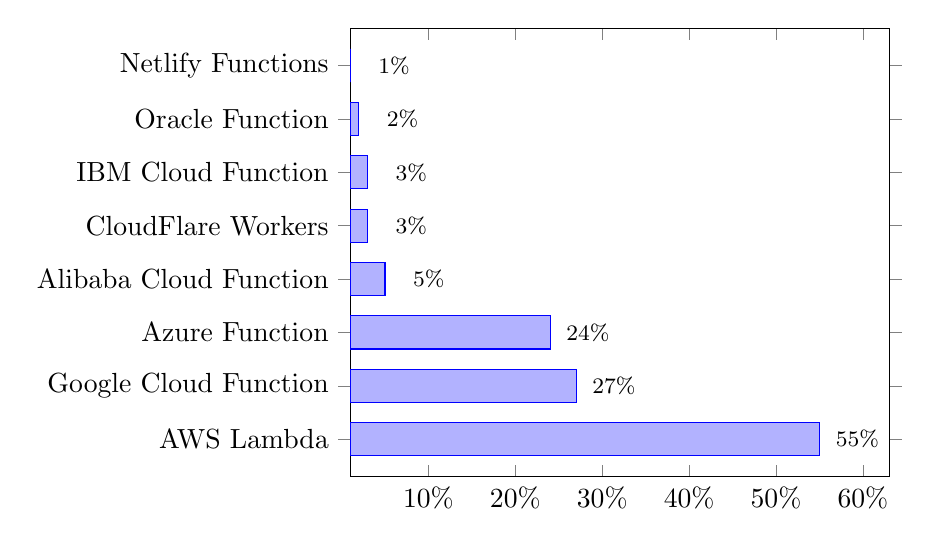
\begin{tikzpicture}
        \begin{axis} [xbar = .05cm,
            bar width = 12pt,
            ytick = data,
            enlarge x limits = {value = .15, upper},
            symbolic y coords={AWS Lambda,Google Cloud Function,Azure Function,Alibaba Cloud Function,CloudFlare Workers,IBM Cloud Function,Oracle Function,Netlify Functions},
            xticklabel={\pgfmathprintnumber\tick\%},
        ]
        
        \addplot coordinates { 
            (55,AWS Lambda) 
            (27,Google Cloud Function) 
            (24,Azure Function)
            (5,Alibaba Cloud Function)
            (3,CloudFlare Workers)
            (3,IBM Cloud Function)
            (2,Oracle Function) 
            (1,Netlify Functions) 
        };
        \addplot[only marks, 
            nodes near coords,         
            every node near coord/.append style={xshift=25pt,yshift=0pt,anchor=east,font=\footnotesize},
            point meta=explicit symbolic,
            ] coordinates { 
            (55,AWS Lambda) [$55\%$]
            (27,Google Cloud Function) [$27\%$]
            (24,Azure Function) [$24\%$]
            (5,Alibaba Cloud Function) [$5\%$]
            (3,CloudFlare Workers) [$3\%$]
            (3,IBM Cloud Function) [$3\%$]
            (2,Oracle Function) [$2\%$]
            (1,Netlify Functions) [$1\%$]
        };     
        \end{axis}    
    \end{tikzpicture}
    \caption{Hosted serverless platform usage according to the CNCF survey \cite{CNCFServerlessSurvey2020}}
    \label{fig:hosted-serverless-platform-share-survey}
\end{figure}

\textbf{Amazon Web Services}, \textbf{Microsoft Azure} and \textbf{Google Cloud Platform} are distinguished as three providers with the biggest market share. Their services are classified into categories and described in more details, altogether with other vendors and companies providing their services in the serverless computing field.

% https://hentsu.com/serverless-computing-aws-vs-azure-vs-gcp-cloud-comparison/
% https://www.datamation.com/cloud/aws-vs-azure-vs-google-2020-cloud-comparison/
% https://www.gartner.com/doc/reprints?id=1-1ZDZDMTF&ct=200703&st=sb

% Categories
% \begin{enumerate}
%     \item Compute
%     \item Data Store (Storage + Database)
%     \item Network and Content Delivery (API management + Hosting)
%     \item Application Integrations (Application Integration + Function Orchestration/Workflow)
%     \item Analytics
%     \item Security and Identity
%     \item Development Tools
% \end{enumerate}

\subsection{Amazon Web Services}

As previously mentioned, Amazon was the company that pioneered the field of serverless computing. Over the years it established the dominant market position, leading in the number of available services characterized by high quality and undergoing constant innovation. AWS is an enterprise ready vendor, highly focused on the public cloud sector providing most comprehensive network infrastructure and data centers.

Moreover, it comes up with rich collection of advanced tools helping developers managing the infrastructure as a code (IaaS) using CloudFormation or AWS Cloud Development Kit improving the maintainability of application architecture as well as developing, building and testing the software by using AWS Serverless Application Model (SAM) which efficiently integrate with other AWS services to ease the development experience. Besides the essential services necessary to develop serverless applications, which are described in more details based on the official documentation \cite{AWSServerlessOffering} below, AWS offers wide range of services oriented towards artificial intelligence and machine learning, that allow to train and deploy machine learning models, analyse documents, images or speach. Among other groups AWS provides services capable of connecting and cooperating with various IoT devices, process multimedia or help managing business processes.

The AWS pricing model is considered as a major difficulty when it comes to accurately estimate the cost of running the service, but most frequently the variety and maturity of services and tooling counterweight that downside.

% https://aws.amazon.com/serverless/

\begin{enumerate}
   \item Compute
   \begin{itemize}
       \item AWS Lambda - First FaaS offering available on the market, that allows to execute the function without provisioning and managing the servers, automatically scaling the solution by running the code in response to an event. AWS Lambda supports Node.js, Python, Go, Java, Ruby, C\# and PowerShell as execution environments as well as any container runtime, charging for the execution with the millisecond granularity and ensuring consistent performance by enabling Provisioned Concurrency.
       \item AWS Fargate - Serverless compute engine for containers also removing the need to manage the servers, eliminating the need to choose instances and scale the cluster capacity, providing appropriate level of isolation and security.
       \item Lambda@Edge - Enable to run the Lambda code at an AWS location closer to the users of the application, utilising the Amazon CloudFront as content delivery network (CDN) to reduce the latency and improve the performance.
   \end{itemize}
   \item Data Store
   \begin{itemize}
       \item Amazon Simple Storage Service (S3) - Object Storage Service offering high data availability, scalability and performance. It enables the storage of a wide range of data for different use-cases such as application data, backups, data lake, websites and other assets ensuring their durability.
       \item Amazon DynamoDB - Flexible, scalable and distributed key-value and document database providing high performance and low-latency data access. Enables data caching, cross-region replication, fault-tolerance and data encryption, being a suitable solution for web and mobile applications.
       \item Amazon Aurora Serverless - Autoscalable and fully managed configuration for Amazon Aurora, which is a relational database compatible with MySQL and PostgreSQL enabling higher performance and availability.
       \item Amazon RDS Proxy - Fully managed and highly-available database proxy for Amazon RDS, which is a service that provides hosting and scaling for other relational databases.
       \item ElastiCache - In-memory data store, compatible with Redis and Memcached suitable for data intensive applications with high throughput and low-latency data access.
   \end{itemize}
   \item Network and Content Delivery
   \begin{itemize}
       \item Amazon API Gateway - Managed services enabling to expose an API and connect with other AWS services providing real-time two-way communication via REST or Websocket API, billed accordingly to usage.
       \item AWS AppSync - Another fully-managed and scalable service capable of defining and handling the two-way communication using GraphQL API handling the heavy-lifting and communicating with other AWS services to store and sync the data.
       \item Amazon CloudFront - Fast, secure and programmable content delivery network (CDN) delivering data such as videos, applications utilising the AWS edge network location to make the service globally scalable and accessible.
   \end{itemize}
   \item Application Integrations
   \begin{itemize}
       \item Amazon Simple Notification Service (SNS) - fully managed publish-subscribe service enabling high-throughput, many-to-many messaging for communication between applications, microservices and application-to-person messaging.
       \item Amazon Simple Queue Service (SQS) - message queuing service allowing to decouple components of the distributed systems in two types - standard (offering high throughput and best effort ordering) and FIFO (designed for ordered messages delivered exactly once).
       \item Amazon EventBridge - Scalable serverless event buss enabling to integrate the incoming messages from other SaaS offerings in real-time with the AWS infrastructure.
       \item AWS Step Functions - Serverless function orchestrator enabling to combine AWS Lambda functions into workflows based on business processes, visualising them and maintaining the application state between execution.
   \end{itemize}
   \item Analytics
   \begin{itemize}
       \item Amazon Kinesis - Offers key capabilities of scalable and fully-managed event streaming service processing and analyzing real-time video, audio and other data streams instantly without necessity to collect the data.
       \item Amazon Athena - Interactive and managed query service for Amazon S3 based on predefined schema, using standard SQL syntax to quickly analyze large-scale datasets
   \end{itemize}
   \item Security and Identity
   \begin{itemize}
       \item AWS Identity and Access Management (IAM) - Required to manage users and groups and their access to AWS services and resources in a secure way, offered without additional cost.
       \item Amazon Cognito - Provides authentication service and identity management that can be easily incorporated with various clients solutions on different platforms.
   \end{itemize}
   \item Development Tools
   \begin{itemize}
       \item Amazon CloudWatch - Service providing application monitoring and observability, gathering logs, metrics and capturing events within the AWS resources. Enable to analyse the environment behaviour, troubleshoot issues and take automate actions based on numerous indicators.
       \item AWS X-Ray - Tool allowing to analyze and debug distributed application behaviour across multiple services based on the request tracing, gathering the execution metric to identify the application issues and performance bottlenecks, available for both development and production applications.
       \item AWS Amplify - Suite of tools and services helping developers build efficient and scalable applications for web and mobile platforms providing possibilities to deploy the statis site, easily manage content or configure the app backends with authentication and data storage.
       \item AWS CodeStar, AWS CodePipeline, AWS CodeBuild, AWS CodeDeploy - Set of tools helping with the automation, continuous integration and deployment workflows for various applications.
   \end{itemize}
\end{enumerate}

\subsection{Microsoft Azure}

Microsoft is the second from the biggest three vendors that started offering its serverless computing services in 2017 by integrating them into the Microsoft Azure platform. It also provides a vast number of services, giving a more flexible and configurable runtime engine supporting more programming languages.

When investing in the serverless field, Microsoft decided to repurpose its existing proprietary software to be available and greatly integrated with the cloud. Microsoft Azure is eager to cooperate with various enterprise companies, especially using their software. Contrary to the AWS, Azure platform can more effectively interoperate with customers' data centers enabling the gradual migration of on-premise software or operate in a hybrid cloud model. Azure platform also provides some powerful DevOps tooling and numerous services integrating machine learning and artificial intelligence, exposing among the others cognitive services, chatbots and document, images and video analysis and recognition.

Nevertheless, customers frequently are not satisfied with the complex pricing model due to complicated software licensing options, that are hard to understand without outside help as well as some of the services are considered less enterprise-ready due to issues with quality of these services, technical support and lacking documentation or when managing and configuring some of them outside of the Azure platform.

Similarly, the current serverless offering is presented in more details according to the information available on the vendor website \cite{AzureServerlessOffering}.

% https://azure.microsoft.com/en-us/overview/serverless-computing/
% https://azure.microsoft.com/en-us/solutions/serverless/#solution-architectures

\begin{enumerate}
   \item Compute
   \begin{itemize}
       \item Azure Functions - FaaS offering from Microsoft, integrating with other services, execution in an event-driven manner and auto-scaling cased on demand. It provide tools for building and debugging functions locally, supporting implementations in .NET Platform (C\#, F\#), Java, Node.js (JavaScript and Typescript), Python and PowerShell, billing the execution on a per second basis.
       \item Azure App Service - Fully-managed platform for building, deploying and scaling web applications written in .NET, Node.js, Java, Python and PHP running in Windows or Linux containers integrating with other services from Azure platform.
       \item Azure Kubernetes Service - Highly-available and secure managed Kubernetes service automatically provisioning serverless infrastructure based on the traffic, utilising open-source tools like Virtual Kubelet for provisioning nodes and KEDA for event processing from various event sources.
   \end{itemize}
   \item Data Store
   \begin{itemize}
       \item Azure Blob Storage - Scalable, secure and durable object storage capable of storing a large amount of unstructured data objects suitable for cloud-native and mobile apps. Providing high availability and geo-replication generating events pushed to other Azure services upon data changes.
       \item Azure Cosmos DB - Fully-managed, globally distributed and multi-modal NoSQL database service, guaranteeing low-latency data access and scalability, exposing APIs for SQL, MongoDB and Cassandra.
       \item Azure SQL Database - Family of SQL cloud databases providing optimized performance, data durability, backups capabilities and adapting to requirement changes.
       \item Azure Cache - Managed in-memory data store which can be utilised as caching layer, providing high throughput and low-latency operation time, scaling according to demand with geo-replication and Redis compatibility
   \end{itemize}
   \item Network and Content Delivery
   \begin{itemize}
       \item API Management - Service enabling API management across cloud and on-premise environments with unified management experience, focused on security and observability with fine-grained data exposition rules and integration with other services.
       \item Azure Content Delivery Network - Secure and reliable content delivery network (CDN) greatly integrated with different services from Azure platform, ensuring proper security level and analytics features.
   \end{itemize}
   \item Application Integrations
   \begin{itemize}
       \item Azure Event Grid - Service handling the message routing from various event sources, working in a publish-subscribe model, ensuring scalability and high-reliability.
       \item Azure Event Hub - Managed, scalable and geo-replicable real-time data streaming service enabling to build dynamic data pipelines, capable of seamless integration with other Azure services.
       \item Azure Service Bus - Reliable and scalable messaging services for a cloud enabling to build communication between decoupled application components and on-premise systems, enabling various messaging models and offline delivery.
       \item Logic Apps - Service enabling developers to build various workflows within containerized environments, integrating external services and enterprise SaaS offerings along with the Azure platform components.
       \item Azure Durable Functions - An extension for Azure Functions enabling them to execute stateful computation in a serverless environment by utilising the Orchestrator that defines the state flow between subsequent functions.
   \end{itemize}
   \item Analytics
   \begin{itemize}
       \item Azure Stream Analytics - Serverless real-time analytics enabling to build streaming pipelines with similar SQL-like syntax integrating with other platform services, including artificial intelligence for more sophisticated use-cases.
   \end{itemize}
   \item Security and Identity
   \begin{itemize}
       \item Azure Active Directory - Service enabling identity management, authentication and authorization capabilities for end users. Enhancing it with single sign-on to multiple SaaS applications, multi-factor authentication functionalities and integration with external identity providers.
   \end{itemize}
   \item Development Tools
   \begin{itemize}
       \item Azure Monitor - Fully managed and scalable monitoring offering integrated with numerous Azure services, providing operational telemetry to analyze the cloud and on-premise services behaviour and performance, allowing to query and visualize the data and trigger alarms based on thresholds or patterns detected by artificial intelligence to proactively notify about anomalies or issues
       \item Azure DevOps - Cloud hosted service providing a fully-fledged set of operational tools such as code repository and task management capabilities, enabling configuration of continuous integration and continuous delivery pipelines along with building artifacts and deploying software to multiple platform or on-premise services.
   \end{itemize}
\end{enumerate}

\subsection{Google Cloud Platform}

Google introduced its serverless products from their cloud offering in 2018 into general availability after a long period in beta. It is noticeable that the Google Cloud Platform offering is not as rich and varied and the services are not as mature and configurable compared with the AWS or Azure catalog.

The vendor is looking to cooperate closely with companies trying to scale quickly and startups rather than large enterprises. Besides the serverless platform, the provider is highly focused on containerization and microservices architecture with the leading in the Kubernetes services along with strong open-source commitments and DevOps-friendly approach. Google Cloud Platform is a leader in fields of artificial intelligence, machine learning and big data offering numerous services and capabilities based on the open-source frameworks and libraries maintained by Google.

The provider gives a better impression to its customers in terms of the ease of setup and user-friendliness of the platform. The pricing model is aimed to be more customer friendly, offering exceptionally flexible contracts appealing to customers interested in using the cloud.

Google Cloud Platform services are presented based on the available offer below \cite{GCPServerlessOffering}.

% https://cloud.google.com/serverless
% https://www.youtube.com/watch?v=4D3X6Xl5c_Y&list=PLIivdWyY5sqKh1gDR0WpP9iIOY00IE0xL&ab_channel=GoogleCloudTech

\begin{enumerate}
   \item Compute
   \begin{itemize}
       \item Cloud Function - FaaS platform from Google enabling to run the code without server management, scalable with the size of workload. Currently it supports Node.js, Python, Go, Java, .Net and Ruby runtimes, priced based on number of invocation and execution duration with granularity to 100ms.
       \item Cloud Run - Scalable and fully-managed container-based execution environment built on top of the Knative open-source project triggered based on various platform events, automatically replicated across multiple regions and billed according to actual usage.
       \item App Engine - Hosting platform for mostly web applications written in Node.js, Java, Ruby, C\#, Go, Python, or PHP responsible for managing the infrastructure and scaling the solution
   \end{itemize}
   \item Data Store
   \begin{itemize}
       \item Cloud Storage - Object storage ensuring security, durability, low latency data access and geo-redundancy enabling to store data across different storage classes characterised with different parameters and cost.
       \item Cloud SQL - Managed and cloud-based relational database service for MySQL, PostgreSQL and SQL Server ensuring reliability and automate database provisioning and storage management.
       \item Cloud Spanner - Database with relational semantics and strong consistency with unlimited scaling, delivering high-performance transactions across regions, automatically handling scaling and sharding
       \item Firestore - Serverless NoSQL document database scaling with the demand with no maintenance overhead, with built-in live synchronization, ACID transactions and offline support. Designed to be used with mobile, web and IoT applications with direct connecting clients, integrating with other Google Cloud Platform services.
       \item Cloud BigTable - Fully-managed and scalable NoSQL database service designed for machine learning and big data services, seamlessly scaling to the storage needs, capable of processing high-throughput data with low latency
       \item Memorystore - Low latency, scalable and secure in-memory service compatible with Redis and Memcached enabling high-availability, automatic failover, patching and monitoring.
   \end{itemize}
   \item Network and Content Delivery
   \begin{itemize}
       \item Cloud Endpoints - Development, deployment and management tool for APIs, providing logging, monitoring, access control and integrations with third party services as identity providers.
       \item Cloud CDN - Globally distributed and reliable content delivery network (CDN) for images, videos, webpages integrating with other services and supporting hybrid and multi-cloud architectures.
   \end{itemize}
   \item Application Integrations
   \begin{itemize}
       \item Cloud Pub/Sub - Messaging event-driven system and streaming analytics, auto-scalable, with no provisioning and cross-zone message replication, enabling in-order messaging with push and pull models
       \item Cloud Tasks - Fully managed service that allows to manage and distribute vast number of distributed tasks asynchronously to build more decoupled applications in microservices architecture that can be scaled independently
       \item Cloud Scheduler - Managed cron job service suitable for batch and big data jobs as well as cloud infrastructure operations, automating management tasks and handling retries in case of failures.
       \item Workflows - Workflow orchestration services across multiple Google Cloud Platform components, focusing on modeling workflow logic, executing them in a reliable way, passing the execution state between particular steps.
   \end{itemize}
   \item Analytics
   \begin{itemize}
       \item BigQuery - Serverless data warehouse based on real-time data stream with autoscaling and managed infrastructure, enabling multi-cloud capabilities, integrated with many tools and services of Google Cloud Platform in the fields of machine learning, artificial and business intelligence.
   \end{itemize}
   \item Security and Identity
   \begin{itemize}
       \item Identity and Access Management (IAM) - Service provides management capabilities for fine-grained access control for Google Cloud Platform resources along with monitoring and auditing them.
       \item Cloud Identity - Service providing unified identity and access management for applications and endpoints, enforce strong security and access control and enable access to thousands of applications via single sign-on
   \end{itemize}
   \item Development Tools
   \begin{itemize}
       \item Cloud Build - Servers as a serverless service for building, testing and deploying artifacts and applications utilising integration and continuous delivery pipelines
       \item Cloud Logging - Real-time log management and analysis services, capable of extracting data from logs and analyzing them in real-time.
       \item Cloud Monitoring - Service enabling to collect metrics from various sources, visualising them, monitor application and services behaviour and integrate with other third party solutions to provide better visibility and observability of the system.
       \item Cloud Trace, Cloud Debugger, Cloud Profiler - Set of tools helping developers with tracing events in the distributed system and collecting numerous metrics, debugging the production application to get more insight into their behavior and profiling the application performance and resource utilisation.
   \end{itemize}
\end{enumerate}

In addition to the Google Cloud Platform services, Firebase \cite{Firebase} is another and independent service backed by Google and based on their cloud platform, providing BaaS components that can be directly integrated with web and mobile clients. All of the services are auto-scalable and with the infrastructure managed on the provider side. The core feature is a real-time document database utilising Firestore underneath, integrating with Cloud Functions, Cloud Storage and providing authentication capabilities. Moreover, the offering includes other components that allow developers to monitor the performance and stability of applications and also analyse the customers behaviour, enable A/B testing and boost their engagement by in-app and cloud messaging.

\subsection{Other cloud providers and services}

\subsubsection*{IBM}
IBM Cloud focuses on helping enterprises migrate to the cloud, extend their capabilities and transform their workloads to be more agile utilising cloud infrastructure. Over the years the company invested in industry-focused cloud services and hybrid cloud market, supporting diverse workloads including SAP, Oracle ERP and newer technologies including machine learning capabilities. Company promotes open-source initiatives to produce the results and portable components that can be used among multiple cloud providers \cite{Gartner}.

In terms of serverless components, IBM Cloud Functions is based on open-sourced Apache OpenWhisk platform, which manages the infrastructure and scaling using Docker containers and can be deployed independently on top of popular container frameworks like Kubernetes, Mesos or OpenShift. The platform supports a programming model in which functions (called Actions) are dynamically provisioned in response to associated events (called Trigger) coming from numerous external sources or HTTP requests. Currently OpenWhisk supports a large number of environments such as Node.js, Go, Java, Scala, PHP, Python, Ruby, Swift or any executable running inside the Docker container \cite{ApacheOpenWhisk}.

\subsubsection*{Alibaba Cloud}

Alibaba Cloud is a cloud provider having strong ties with Chinese public sector as well as cooperation with numerous companies operating in the China and Southeast Asia region. The cloud vendor supports its clients with cloud migration and helps traditional enterprises to build their presence in digital platforms. Most of its clients reported satisfaction with platform solutions, but the limitations can be noticed in not as broad international offerings compared to the services available in China region as well as discrepancies in documentation and functionalities availability \cite{Gartner}.

The Function Compute is a serverless FaaS offering with a pay-as-you-go model, managed and scaled by the cloud provider in response to events incoming from various data sources. It supports mainly Node.js, Python, Java, PHP, C\# and custom runtimes in containers. The cloud platform provides two function instances - the flexible functions and instances with higher specifications for better performance, additionally vendors offer reserved instances that are always on and reduce the cold start \cite{AlibabaFunctionCompute}.

\subsubsection*{Cloudflare}

Cloudflare is a company providing services in areas of web infrastructure and website security such as content delivery network, domain name server services and internet security field serving as reverse proxy for websites. It also provides numerous analytics that gives insight into transfer speed, incoming traffic from unique users and their geographic location.

From serverless offerings Cloudflare Workers is a FaaS platform based on edge computing providing high-performance. The solution is also managed, auto-scalable and billed in a pay-per-use model as other serverless offerings, but the difference is the Cloudflare edge network routes the request to the closest location, where the function is executed limiting the latency and providing high availability. Currently the platform supports Node.js, Rust, C, and C++ as an execution runtimes \cite{CloudflareWorkers}.

\subsubsection*{Oracle}

Oracle Cloud is expanding its worldwide presence and their cloud services into numerous regions, developing hyperscale cloud architectures that are competitive with other, more-established cloud providers. The vendor tends to cooperate more closely with enterprises using its business applications and enable to incorporate and integrate them within the cloud platform. All of the cloud offerings are available in multiple regions with the same capabilities \cite{Gartner}.

Oracle Cloud Functions are offered in pay-as-you-go model, managed and scaled by the provider also and they are based on the open-source Fn Project and CloudEvents which is an open-source specification for describing event data. It supports Go, Java, Node.js, Python, Ruby and C\# runtimes and custom runtimes using Docker to execute the functions. The platform is vendor-agnostic and can be also executed in private and hybrid cloud \cite{FnProject}.

\subsubsection*{Netlify}

Netlify is offering hosting and serverless backend services for static websites and web applications. The deployment process is easy and convenient for developers, which can connect Git repository with the platform enabling automatic continuous deployment triggered with every code change. Netlify quickly extended their portfolio with other services such as serverless form submission, user identity management, analytics and also their own, headless content management system which can be utilised by dynamic web applications.

Currently the offer also includes serverless functions powered by AWS Lambda, that can be automatically provisioned when the platform detects the configuration in the linked repository. The Netlify Functions can be triggered based on HTTP request to the defined API or form submission, as well as enabled to run asynchronous processing in Background Functions with longer execution time. Altogether with the whole platform, it allows developers to quickly and easily setup the production environment for the web application or static website without any operational knowledge \cite{NetlifyFunction}.

\subsection{Open-source alternatives}

The benefits of serverless architecture such as cost reduction and eliminating the need of infrastructure management became an appealing argument to use it. Nevertheless, some companies invested heavily in their hardware infrastructure or are afraid of the vendor lock-in or computation restriction of the public cloud platforms. Open-source frameworks are promising to overcome these limitations and manage the serverless components on self-hosted or hybrid clouds.

According to aforementioned survey conducted by CNCF \cite{CNCFServerlessSurvey2020} the the most popular solution in the category of installable software for serverless function execution is newly added Knative (claimed to be used by 27\% of respondents), while OpenFaaS maintains its popularity (used by 10\% of interviewee) with Kubeless (mentioned by 5\% of respondents).

All of the projects are based on the Kubernetes as a portable and extensible platform enabling declarative configuration and management for containerized environments. Serverless frameworks rely on it to orchestrate and manage the serverless functions inside containers, schedule their executions, provide service discovery and replication. Each of the open-sourced serverless frameworks approach the container orchestration slightly differently. For example, OpenFaas provides its own API Gateway providing access to the function, collecting metrics and scaling the solution, while others like Knative utilise third-party Ingress Controller for Kubernetes and manage the scaling by Queue-Proxy Container, passing the events to functions inside the pod. Several articles consider the viability and quality of services for the open-source serverless platforms \cite{OpenSourceServelessPerformance}, considering also interesting possibilities of utilising serverless in edge computing \cite{OpenSourceServelessEdge}.

Nevertheless, utilising open-source platforms raises questions about maturity of these frameworks and introduces another set of challenges, which need to be researched and addressed. Based on the previously mentioned articles some of the serverless platforms show issues with scaling, lack of it predictability and guarantees ensuring good quality of service. Each of the frameworks enable default fault tolerance for containers runtime limited to retrying the execution, which sometimes may be not suitable. Above all public cloud providers tend to supply various tools and services that support developers with log aggregation, monitoring, alerting and distributed tracing across the distributed system, which requires manual integration in the open-source alternatives. Public cloud vendors offer not only the FaaS platforms, but also provide a large variety of BaaS components that can be integrated with serverless functions to build fully-fledged applications and services. Contrary to the open-sourced alternatives, which focus solely on the FaaS platforms. While the other components could be also self-hosted, integration with them as well as scaling requires manual management on the customer side, increasing the amount of work that needs to be done to maintain the services quality and going against the idea of serverless.

\subsection{Comparison of serverless providers}

% TODO:rb
TBD?

% - comparable offering, but when diving into internals, the differences may be more visible if it comes to maturity of services
% - different market share? 
%     - Azure towards enterprise, hybrid, and private clouds
%     - AWS towards public cloud
%     - GCP - ok with startups and smaller companies, open source and ML/AI/BigData

% - available services, 
% - approaches to develop serverless apps, 
% - can Open-Source replace providers?
% - table comparison ???

% https://thenewstack.io/serverless-on-public-cloud-the-ultimate-showdown/
% https://www.datadoghq.com/state-of-serverless/

\section{Example use cases}

% https://pages.awscloud.com/rs/112-TZM-766/images/Asset2-optimizing-enterprise-economics-serverless-architectures.pdf - examples
% https://www.simform.com/serverless-aws-lambda-examples/
% https://dashbird.io/blog/companies-using-serverless-in-production/

% \cite{ServerlessArchitectureOnAWS}
% - suitable for some types of processing - reference to benefits
% - serverless is suitable for building whole systems, create isolated components or implement specific and granular tasks - serverless can be applied to small and large tasks
% - serverless is not only about processing by lambdas, but also 3rd party services, which amke possible to cut down the work

\subsection{Application backend}

% https://livebook.manning.com/book/serverless-architectures-on-aws/chapter-2/36 - CloudGuru

Serverless technologies are an appropriate solution for building scalable application backends for all kinds of web, mobile and desktop applications. They are favorable for this use-case, because the infrastructure management can be effectively automated ensuring dynamic scaling to meet uneven demand, with proportional and predictable billing. Despite the fact that serverless technologies are a relatively new approach to building services, some of the companies already used it to power large applications.

To build the application backend, serverless functions are used to transform the data representing the application logic together with other third party services capable of persisting data or exposing some desired functionalities. The API Gateway provides uniform access to various serverless functions using REST API, ensuring mapping between requests and respective serverless functions, enabling integrations with other services responsible for authentication and authorisation. Sending a request to the API can lead to execution of one or more serverless functions containing custom business logic and communicating respectively with other services. It is also possible that the frontend application can communicate directly with external components bypassing the API Gateway. Nevertheless, it is essential to handle the communication in a secure manner for example using the delegation tokens \cite{ServerlessArchitectureOnAWS}.

\begin{figure}[h]
    \centering
    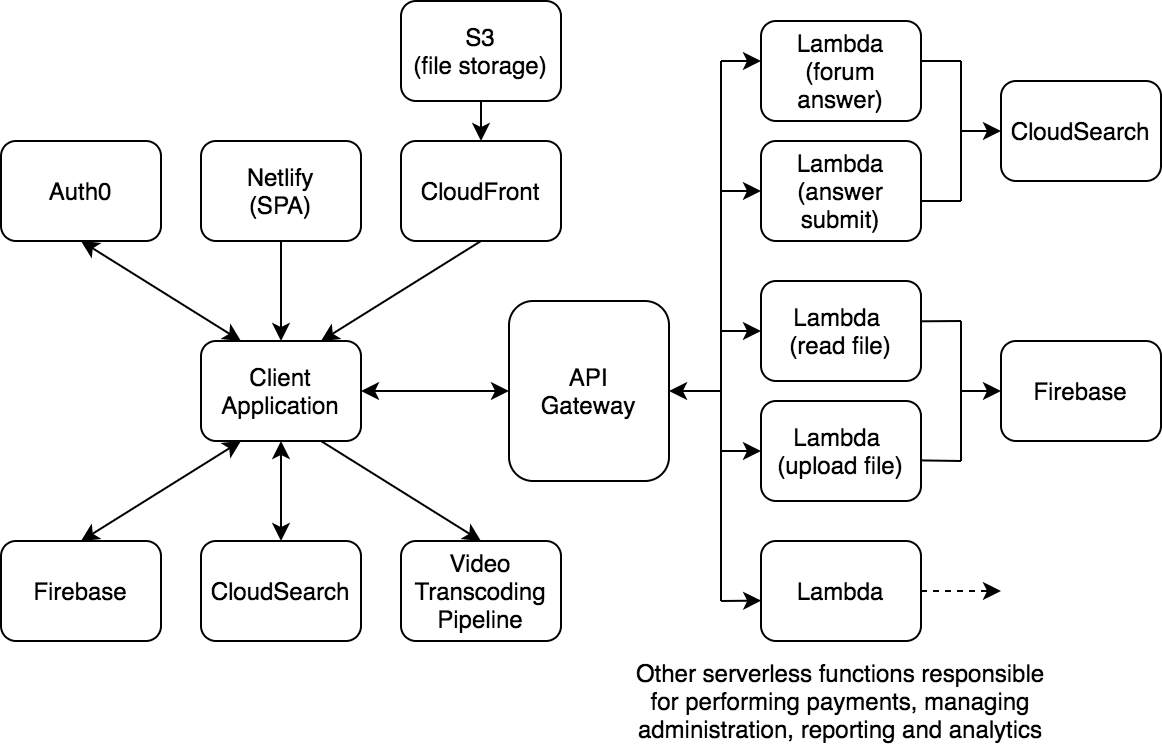
\includegraphics[width=0.8\textwidth]{assets/02-serverless/CloudGuruArchitecture.png}
    \caption{CloudGuru platform architecture}
    \label{fig:cloudguru-architecture-diagram}
\end{figure}

CloudGuru, which is an online educational platform dedicated to people interested in learning numerous cloud related topics, is a good example of such a use-case. Core features of the platform include streaming large selection of video courses, interactive quizzes and practice exams, real-time discussion forum and integrations with third party services allowing users to buy access to the courses.

The architecture of the e-learning platform utilises services of several cloud providers. Frontend of the web application built as a Single Page Application is hosted on Netlify, which acts as a Content Delivery Network (CDN) for the platform client. Auth0 service is responsible for registration and authentication functionalities and provides delegation tokens for client application to communicate directly and securely with other services. Firebase is used as a primary database, capable of updating clients in real-time using websockets to push updates to the client applications. Questions and answers submitted by users to the forum are persisted in the Firebase, later the data is sent to AWS CloudSearch which is indexing it for further searching purpose, enabling users to find information easier. Instructors can upload videos directly to S3 bucket, which triggers the video transcoding pipeline. Users can watch the videos served via CloudFront acting as a CDN if they call the lambda function beforehand, giving them the permission to access the video assets for a limited period of time.

\subsection{Event-driven data processing}

% https://livebook.manning.com/book/serverless-applications-with-node-js/chapter-15/1 -  CodePen, MindMup
% https://www.doc.ic.ac.uk/~rbc/papers/fse-serverless-17.pdf ~ MindMup in more details

Serverless has also found application in numerous media conversion and transcoding as well as various data processing tasks. When the new file is inserted to the bucket responsible for data storage, it can trigger a serverless function passing the necessary data and file as an event to perform the processing. Such an event-driven approach is suitable for building pipelines for data-processing tasks, billed only for the lambda execution time and other BaaS components usage to transfer, transform or extract some information, if applicable \cite{ServerlessArchitectureOnAWS}.

\begin{figure}[h]
    \centering
    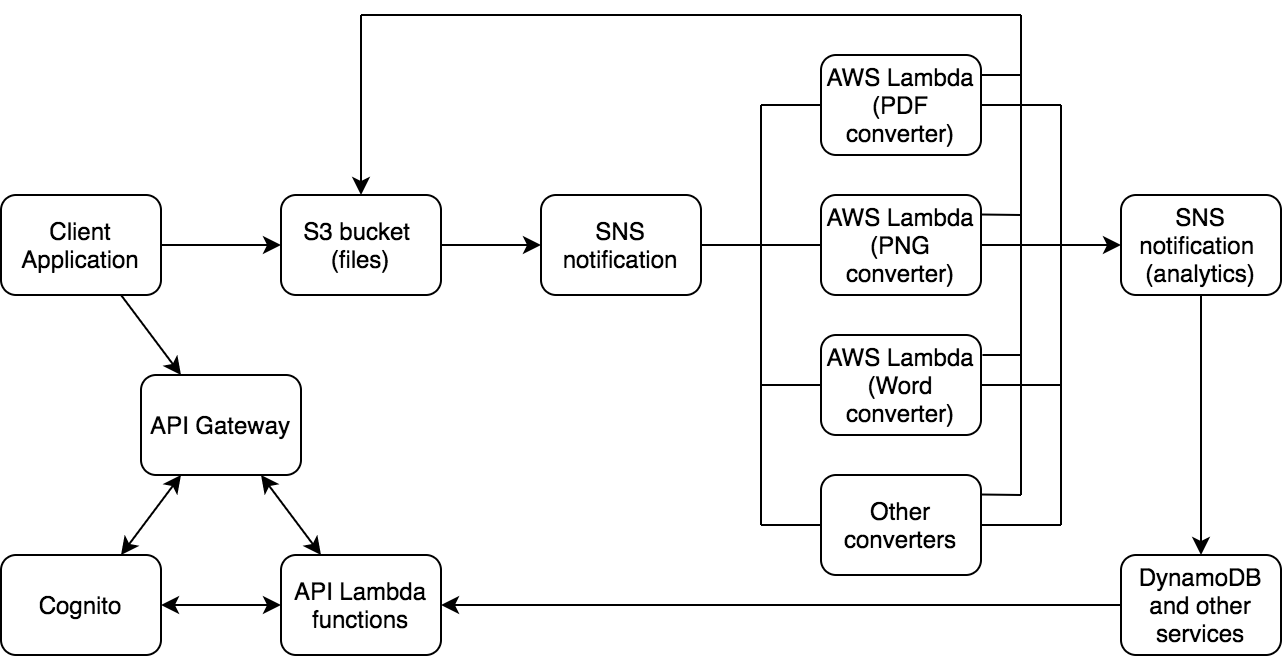
\includegraphics[width=0.8\textwidth]{assets/02-serverless/MindMupArchitecture.png}
    \caption{MindMup platform architecture for file export}
    \label{fig:mindmup-architecture-diagram}
\end{figure}

An example of such serverless use is MindMup, which is a popular web application mind mapping tool running in the web, developed with just 2 person team. The event-driven data processing is utilised in the case when user wants to export prepared diagram to some read-only format such as PDF, Word document, presentation or text file. The web application works as interactive user interface, upon user requests to export the diagram, it calls the Lambda placed behind the API Gateway to generate the presigned URL, which can be used for a short period of time to insert the file inside the S3 bucket, directly from the client application. It sends an event to the Amazon Simple Notification Service (SNS) triggering the appropriate function responsible for export to a particular file format. Each of the exporters have different requirements, for example CPU and memory usage for PDF exporter is much higher than for others or Microsoft Office exporters require usage of libraries written in Java. Moreover, some of the extensions such as Markdown are not as frequently selected by users as others. When the processing is complete, the output of the process is put back in the S3 bucket, where the users can access it. Additionally the event is sent to SNS which triggers other services such as DynamoDB that are listening to that topic to save some information for analytics purposes.

The company admits that initially, the service responsible for exporting was running on the Heroku platform in the containerised environment, but after migration to the AWS Lambda they've noticed significant cost reduction even with the growth of the platform usage by the clients \cite{ServerlessApplicationsWithNodejs}.

\subsection{Real-time stream processing}

Serverless architecture also found application in the data ingestion tasks from numerous data sources such as logs, system events, transactions or social media feeds that need to be analyzed, aggregated and stored. Utilising BaaS components capable of event stream aggregation over time with the serverless function which can be configured to run when the specific number of records (forming a batch of records) is available. Such a messaging pattern is popular in distributed systems and allows decoupling the services and provides reliability by storing the messages in the queue when the consuming service cannot process more data at the moment, additionally providing retrying mechanism in case of failures \cite{ServerlessArchitectureOnAWS}.

\begin{figure}[h]
    \centering
    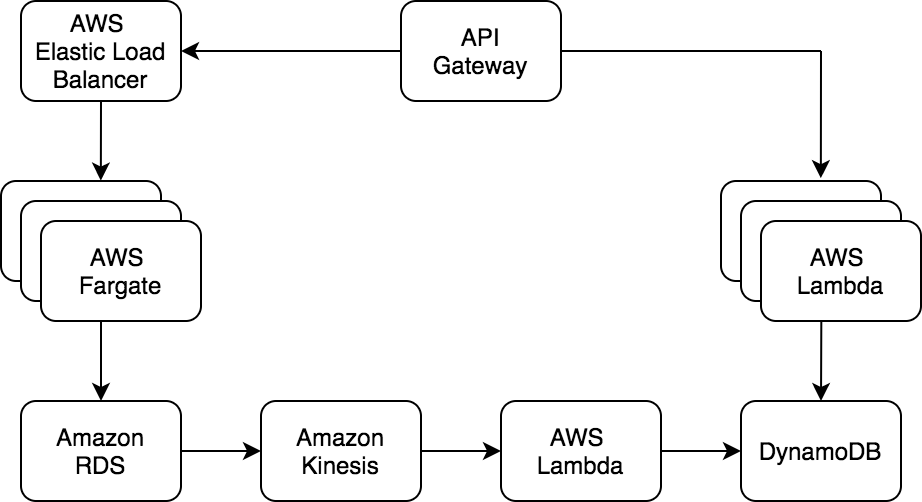
\includegraphics[width=0.7\textwidth]{assets/02-serverless/TemenosArchitecture.png}
    \caption{Temenos platform architecture}
    \label{fig:temenos-architecture-diagram}
\end{figure}

Temenos as one of the largest banking software providers is using such a pattern along with other serverless technologies in their T24 Transact banking system to achieve a highly elastic solution with low maintenance cost. It supports a large number of interactions and transactions between banking customers worldwide and due to leveraging the platform and managed services it reports that even the unpredictable workloads due to peaks in the market are handled efficiently. All the requests coming to the systems are getting through the AWS API Gateway which passes them the AWS Elastic Load Balancer (ELB) responsible for routing the requests to the proper container instance on AWS Fargate. The application running inside the container based on the request, performs the business actions and persists the result in Amazon Relational Database Service (RDS) that is an Online Transactional Processing Database (OLTP) designed to process the transactions effectively. Later the stream of data events and more complex business events is pushed from Amazon RDS to Amazon Kinesis which aggregate the data and triggers the AWS Lambda responsible for processing it to build a query-optimized data model that is stored in DynamoDB. When the banking system users want to query the data, they perform a request that goes from API Gateway to AWS Lambda that query the read-optimized data model from DynamoDB \cite{ThisIsMyAchitectureTemenos}.

\subsection{IoT applications}

With the growth of smart homes popularity along with other devices that are meant to help people, IoT devices started incorporating more sophisticated technologies to support people on a daily basis. iRobot is a leading company in terms of designing and building smart robots helping people around their household with the Roomba robotic vacuums as their most popular product. Besides robotics the company provides iRobot HOME application which enables customers to interact with their smart home devices.

\begin{figure}[h]
    \centering
    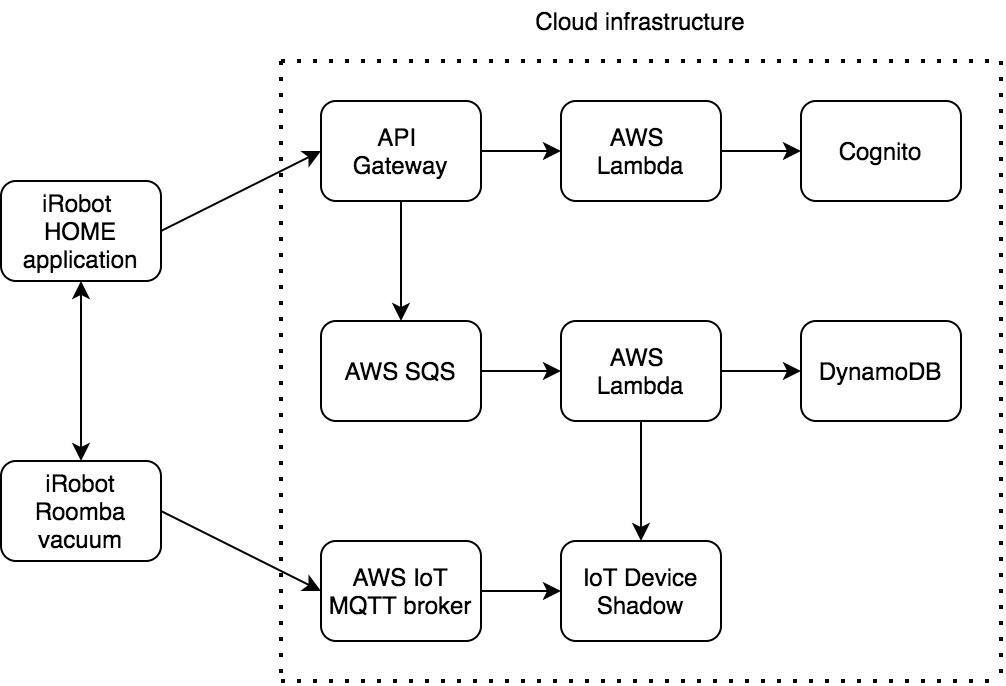
\includegraphics[width=0.7\textwidth]{assets/02-serverless/iRobotArchitecture.png}
    \caption{iRobot solution architecture for smart robots}
    \label{fig:irobot-architecture-diagram}
\end{figure}

AWS IoT is an entry point for the Roomba vacuums to connect them with the cloud. For the communication purposes MQTT is used, which is a lightweight publish-subscribe protocol for IoT devices. The AWS IoT Shadow Device enables asynchronous communication mechanism, enabling the robot to work properly without the constant communications with the cloud. When the smart vacuum finishes its job, its data is synchronized with the cloud, which allows users to update the cleaning schedule according to changes made by them via the iRobot HOME application. Along with the AWS IoT developers can define additional IoT Rules that enable the device to connect with other services in the cloud, for example to update the device status along with its parameters, informing users that the vacuum tank is full. Moreover, the gathers additional information about usage and home mapping better plan their tasks and manage the battery power \cite{ServerlessIoTatiRobot}.

Developers and designers of the robotics solutions observed many benefits related with the utilisation of cloud vendors services and the serverless paradigm, mentioning the scalability of the solution without need to manage infrastructure and significant cost reduction, while preserving the proper level of security and data privacy \cite{AWSIRobotIoT}.

% \cite{ServerlessArchitectureOnAWS}

% - bot - app/script running automated tasks for other services
% - responding to commands, carry out small tasks, send reports and notifications

% https://www.researchgate.net/publication/323314352_Case_Study_Building_a_Serverless_Messenger_Chatbot

% ---

% A Review of Serverless Use Cases and their Characteristics - in depth analysis of several cases using serverless architecture (recommended)
% https://arxiv.org/pdf/2008.11110.pdf

% Evaluation of Production Serverless Computing Environments - benchmark
% https://www.researchgate.net/profile/Hyungro-Lee/publication/324362882_Evaluation_of_Production_Serverless_Computing_Environments/links/5b9c1d84a6fdccd3cb579eca/Evaluation-of-Production-Serverless-Computing-Environments.pdf